\documentclass[sigconf,review, anonymous]{acmart}
\acmConference[ESEC/FSE 2018]{The 26th ACM Joint European Software Engineering
Conference and Symposium on the Foundations of Software Engineering}{4-9 November, 2018}{Lake Buena Vista, Florida, United States}

\usepackage[norelsize,linesnumbered,ruled,vlined]{algorithm2e}

%\usepackage[latin1]{inputenc}
\usepackage{graphicx}
%\usepackage{algorithm}
\usepackage{algorithmic}
\usepackage{multirow}
\usepackage{longtable}
\usepackage{rotating}
\usepackage{enumerate}
%\usepackage{slashbox}
%\usepackage{amsthm}
\usepackage{amsmath}
\usepackage{xcolor}
\usepackage{epstopdf}
\usepackage{subfigure}
\usepackage{listings}
\usepackage{xcolor}
\usepackage{url}
\usepackage{caption}
\usepackage{hyperref}
\usepackage{slashbox,multirow}
\usepackage{flushend}
%\reference alignment
\definecolor{keywordcolor}{rgb}{0,0,1.0}
\definecolor{lightgreen}{rgb}{0,0.8,0}
\definecolor{webgreen}{rgb}{0,0.5,0}

\newcommand{\hytt}[1]{\texttt{\hyphenchar\font=\defaulthyphenchar #1}}
\newtheorem{definition}{Definition}
\newtheorem{pattern}{Anti-pattern}
%\renewcommand{\algorithmicrequire}{\textbf{Input:}}
%\renewcommand{\algorithmicensure}{\textbf{Output:}}

% Copyright
%\setcopyright{none}
%\setcopyright{acmcopyright}
%\setcopyright{acmlicensed}
%\setcopyright{rightsretained}
%\setcopyright{usgov}
%\setcopyright{usgovmixed}
%\setcopyright{cagov}
%\setcopyright{cagovmixed}

\lstset{
  language=Java,
  alsolanguage= XML,
  tabsize=4, %
  frame=, %把代码用带有阴影的框圈起来
  %rulesepcolor=\color{red!20!green!20!blue!20},%代码块边框为淡青色
  keywordstyle=\color{red!20!green!20!blue!20}, %代码关键字的颜色为蓝色,粗体
  showstringspaces=false,%不显示代码字符串中间的空格标记
  stringstyle=\ttfamily, % 代码字符串的特殊格式
  keepspaces=true, %
  breakindent=22pt, %
  %frame=single,
  numbers=left,%左侧显示行号 往左靠,还可以为right,或none,即不加行号
  stepnumber=1,%若设置为2,则显示行号为1,3,5,即stepnumber为公差,默认stepnumber=1
  %numberstyle=\tiny, %行号字体用小号
  numberstyle={\color[RGB]{0,204,0}\tiny} ,%设置行号的大小,大小有tiny,scriptsize,footnotesize,small,normalsize,large等
  numbersep=8pt,  %设置行号与代码的距离,默认是5pt
  commentstyle={\color{green}\tiny},%浅灰色的注释
  basicstyle=\footnotesize, % 这句设置代码的大小
  showspaces=false, %
  flexiblecolumns=true, %
  breaklines=true, %对过长的代码自动换行
  breakautoindent=true,%
  breakindent=4em, %
  %aboveskip=1em, %代码块边框
  tabsize=2,
  showstringspaces=false, %不显示字符串中的空格
  fontadjust,
  framextopmargin=2pt,framexbottommargin=2pt,abovecaptionskip=-3pt,belowcaptionskip=3pt,
  xleftmargin=1em,xrightmargin=1em, % 设定listing左右的空白
}

\lstset{language=[AspectJ]Java,
basicstyle=\footnotesize,
keywordstyle=\color{keywordcolor}, %\underbar,
identifierstyle=,
commentstyle=\color{lightgreen} \textit,
stringstyle=\ttfamily,
showstringspaces=false,
captionpos=b
}


% DOI
\acmDOI{10.475/123_4}

% ISBN
\acmISBN{123-4567-24-567/08/06}

%Conference
\acmConference[]{ESEC/FSE'18}{November 04-09, 2018}{Florida, USA}
\acmYear{2018}
\copyrightyear{2018}


%\acmArticle{4}
\acmPrice{15.00}


% These commands are optional
%\acmBooktitle{Transactions of the ACM Woodstock conference}
%\editor{Jennifer B. Sartor}
%\editor{Theo D'Hondt}
%\editor{Wolfgang De Meuter}



\begin{document}
\title{ServDroid: Detecting Service Usage Inefficiencies in\\  Android Applications}
%\titlenote{Produces the permission block, and copyright information}
%\subtitle{Extended Abstract}
%\subtitlenote{The full version of the author's guide is available as \texttt{acmart.pdf} document}

%\iffalse
\author{Wei Song, Jing Zhang}
%\authornote{Dr.~Trovato insisted his name be first.}
\orcid{0000-0002-4324-3382}
\affiliation{%
  \institution{School of Computer Science and Engineering\\Nanjing University of Science and Technology}
  \streetaddress{Xiaolingwei 200}
  \city{Nanjing}
  %\state{Ohio}
  \country{China}
  \postcode{210094}
}
\email{wsong@njust.edu.cn}

\author{Jeff Huang}
%\authornote{This author is the one who did all the really hard work.}
\affiliation{%
  \institution{Parasol Laboratory\\Texas A\&M University}
  %\streetaddress{1 Th{\o}rv{\"a}ld Circle}
  \city{College Station, TX}
  \country{USA}}
\email{jeff@cse.tamu.edu}

% The default list of authors is too long for headers.
\renewcommand{\shortauthors}{}

%\fi

\begin{abstract}
Services are frequently-used components in Android applications, which are responsible for performing time-consuming operations on the background. While services play a crucial role, our study finds that, service usage in practice is not so efficient as expected, reducing the performance of applications, e.g., unnecessary resource occupation and energy consumption. In this paper, according to the service lifecycle, we first formulate four anti-patterns that result in service usage inefficiencies, including premature create, late destroy, premature destroy, and service leak. Since these service usage efficiency bugs do not cause application crashes, it is difficult for existing testing approaches to find them. To this end, we present a static analysis approach, \textsf{ServDroid}, to detect such efficiency bugs in Android applications and output the callers of the services to facilitate debugging. We apply \textsf{ServDroid} to 45 popular real-world Android apps, and surprisingly find that service usage inefficiencies are pervasive.
\end{abstract}

%
% The code below should be generated by the tool at
% http://dl.acm.org/ccs.cfm
% Please copy and paste the code instead of the example below.
%
\begin{CCSXML}
<ccs2012>
<concept>
<concept_id>10011007.10011074.10011099.10011102</concept_id>
<concept_desc>Software and its engineering~Software defect analysis</concept_desc>
<concept_significance>500</concept_significance>
</concept>
<concept>
<concept_id>10011007.10011074.10011099.10011102.10011103</concept_id>
<concept_desc>Software and its engineering~Software testing and debugging</concept_desc>
<concept_significance>500</concept_significance>
</concept>
</ccs2012>
\end{CCSXML}

\ccsdesc[500]{Software and its engineering~Software defect analysis}
\ccsdesc[500]{Software and its engineering~Software testing and debugging}

\keywords{Android app, background service, usage inefficiency, service leak, static analysis}


\maketitle

\section{Introduction}
Mobile applications (apps) are now eating the world. Millions of apps are available on Google Play Store and Apple App Store, and many apps have millions or even billions of downloads. The improvement of computation and memory capacity of mobile devices allows developers to design increasingly powerful and complex apps. On the other hand, more complex apps usually involve more bugs and vulnerabilities, which significantly impact the release and adoption of apps. Thus, the quality of mobile apps receives an increasing attention~\cite{ReavesBGABCDHKS16,AnandNHY12,MachiryTN13,ChoiNS13,LiuXC14,BanerjeeC0R14,LiuXCL14,HechtBRMD15,BehrouzSBM16,MirzaeiGBSM16,SuMCWYYPLS17}.

Testing is an effective means to find bugs and to improve the quality of apps.
Since Android is popular and open-source, many testing approaches are presented
for Android apps. However, most of them focus on GUI testing of foreground
activities~\cite{monkey,AnandNHY12,MachiryTN13,ChoiNS13,MirzaeiGBSM16,BaekB16,SuMCWYYPLS17,SongQH17},
whereas background services have received few research
attention~\cite{ZhangLLC17}. Services are Android components, performing
long-running tasks that involve few or no user interactions, e.g., file I/O,
music playing, network transaction~\cite{Androidservice}. A service executes on
the main thread of the calling component's process, and thus a new thread is
often created to perform the long-running operations. Services in Android fall
into two categories: system services and app services. Our work focuses on the
latter. According to how app services are used in the code, they can be further
divided into three types: \textit{started services}, \textit{bound services},
and \textit{hybrid services}.
% kinds: local services and remote services. Local services are defined by the app itself whereas remote services are from other apps running on the same device.

Although app services usually do not have user interface, they can keep running
even when the device screen is shut down. As a consequence, if an app involves
service-related bugs, not only the functionalities of the app but its
performance (e.g., resource utilization, energy consumption) can be affected.
In this paper, we focus on service usage inefficiencies (a type of
non-functional bugs) that do not immediately lead to app crashes, but
have a significant impact on the performance of the app.
%This problem has received little attention~\cite{ZhangLLC17} in the literature.
Since such bugs do not cause app crashes, existing testing methods do
not work well in detecting them. Although there exists work on non-functional
testing (mainly energy testing) of apps~\cite{LiuXC14,BanerjeeC0R14,LiuXCL14,BehrouzSBM16,JabbarvandM17}, the
oracle-based on performance indicators are generally more expensive and more
labour-intensive than functional testing~\cite{BehrouzSBM16}.

%Therefore, a large proportion of app energy consumption is caused by background services~\cite{}.

To address this problem, instead of using testing, we first propose four
anti-patterns to facilitate the analysis of service usage
efficiency bugs. These anti-patterns are all defined based on the lifecycle
of services~\cite{Androidservice} and are distilled from our manual analysis
of real-world Android apps. The anti-patterns are described below:
\begin{itemize}
  \item {\bf Premature create} refers to the situation that a
service is created too early before it is really used. Hence, the service is in
an idle state beginning from its create to its real use, occupying unnecessary
memory and consuming unnecessary energy.
\item  {\bf Late destroy} refers to the situation
that a service is destroyed too late after its use. Similarly, the service is in
an idle state beginning from the end of its final use to the moment it is destroyed.
\item {\bf Premature destroy} refers to the situation that a service is initiated by a
component (caller) but it is destroyed before another component begins to use
it. Consequently, the service should be created again to fulfil the new request.
\item {\bf Service leak} refers to the scenario that a service is never destroyed
after its use, even when the apps which initiate the service terminate.
\end{itemize}

% We observe from real-world apps that these four kinds of efficiency bugs are
% common.
For each of the four service usage anti-patterns, we then propose a static
analysis technique to automatically detect its instances (concrete efficiency
bugs matching the anti-pattern) in an app.
% The analysis is based on
% \textsf{Soot}~\cite{sootpaper}\footnote{https://github.com/Sable/soot}, a
% framework for transforming and analyzing Java and Android applications.
Our approach takes an app (APK file) as input and transforms the APK files into
Jimple based on Soot~\cite{sootpaper}. It then constructs a
context-insensitive inter-procedural control flow graph of the app and uses
dominator analysis and successor analysis to find the service usage efficiency
bugs.
Finally, it reports all the
detected service usage efficiency bugs as well as the components (callers) that
initiate the services to facilitate debugging.

We implemented our approach in an open-source tool \textsf{ServDroid}. The tool
is written in Java and is publicly available (links are omitted due to double-blind review).
To investigate the service usage efficiency bugs in real-world apps, we apply
\textsf{ServDroid} to a total of 45 the most popular free Android apps listed on
Wikipedia\footnote{https://en.wikipedia.org/wiki/List\_of\_most\_downloaded\_Android\_applications (accessed in Nov 2017)}.
The downloads of these apps are all over 500 million. Our experiment shows that
service usage efficiency bugs are surprisingly pervasive in the most popular
real-world apps: 42 (93.33\%) apps involve at least one kind of service usage
efficiency bugs; each app has on average 9.6 service usage efficiency bugs.
Our empirical evaluation indicates that service usage inefficiencies are
severe in practice, but the developers have not yet realized their severity.

%The identified bugs are validated through manual analysis or real phone testing, and some of the bugs are confirmed by developers. Our study takes the first step to address these problems, which can inspire the follow-up research on debugging and repairing such bugs.

In summary, the key contributions of this paper are:
\begin{enumerate}
\item According to the service lifecycle, we formulate four service usage
anti-patterns that may lead to unnecessary resource occupation and energy consumption.
\item Based on the anti-patterns, we present a static analysis approach to
detect the service usage efficiency bugs. To our best knowledge, our work
is among the first to detect service usage inefficiencies in mobile apps.
\item We develop an open-source tool, \textsf{ServDroid}, which can
automatically detect service usage efficiency bugs and also help debugging
them.
\item We conduct an empirical study on 45 most downloaded free Android apps,
the results of which demonstrate that the service usage inefficiencies are pervasive in practice.
\end{enumerate}

The rest of the paper is organized as follows. Section~\ref{background} gives an
introduction to the three types of app services.
Section~\ref{antipatterns} formulates the four anti-patterns that lead to
service usage efficiency bugs.
Section~\ref{approach} presents our static analysis for detecting instances
of such anti-patterns.
Section~\ref{evaluation} reports the results of our empirical study.
Section~\ref{relatedwork} positions our approach in the related work, and
Section~\ref{conclusion} concludes the paper.

\section{Background}\label{background}
Along with \textit{activities} (user interfaces),
\textit{broadcast receivers} (mailboxes for broadcast), and \textit{content providers} (local database servers), services (background tasks) are fundamental components in Android apps. To ease the understanding of service usage anti-patterns, we introduce the lifecycle of app services and how they are used~\cite{Androidservice}.

To define an app service, one should inherit the \hytt{Service} class provided by Android, and overwrite corresponding methods of \hytt{Service}, e.g., \hytt{onStartCommand(Intent, int, int)}, \hytt{onBind()}, etc. A service is started in the app by an asynchronous message object which referred to as \textit{intent}. Accordingly, a service declared by a <service> tag in the AndroidManifest XML file of the app ought to have the attribute <intent-filter> which indicates the intents that can start it.  The attribute <exported> indicates the components of other apps can invoke or interact with it. The attribute <isolatedProcess> indicates whether the service is executed in an isolated process. Services can be used in three manners, corresponding to three types of app services: \textit{started service}, \textit{bound service}, and \textit{hybrid service}.

\begin{figure}
  \centering
  \subfigure[]{
    \includegraphics[scale=0.5]{started.eps}}
  \subfigure[]{
    \includegraphics[scale=0.5]{bound.eps}}
  \caption{Service lifecycle of Android apps: (a) started service, (b) bound service.}
\label{fig_lifecycle}
\end{figure}

\textbf{Started service}. The lifecycle of a started service is shown in Figure~\ref{fig_lifecycle}a, which is explained as  follows. A started service is started via \hytt{Context.startService()} which triggers the system to retrieve the service or to create it via the \hytt{onCreate()} method of the service if the service has not been created before, and then to invoke the \hytt{onStartCommand(Intent, int, int)} method of the service. The service keeps running until \hytt{Context.stopService()} or the \hytt{stopSelf()} method of the service is invoked. It is worth mentioning that if the service is not stopped, multiple invocations to \hytt{Context.startService()} result in multiple corresponding invocations to \hytt{onStartCommand()}, but do not create more service instances, that is, the service (instance) is shared by different callers. Once \hytt{Context.stopService()} or \hytt{stopSelf()} is invoked, the service is stopped and destroyed by the system via calling the \hytt{onDestroy()} method of the service, no matter how many times it was started.  However, if the \hytt{stopSelf(int)} method of the service is used, the service will not be stopped until all started intents are processed. Note that the started service and the components which start it are loosely-coupled, i.e., the service can still keep running when the components are destroyed.

\textbf{Bound service}. The lifecycle of a bound service is shown in Figure~\ref{fig_lifecycle}b, which is explained in the following. Since started services cannot interact with the components which start them, bound services are presented, which can send data to the launching components (clients). The client component can invoke \hytt{Context.bindService()} to obtain a connection to a service. Similarly, this creates the service by calling  \hytt{onCreate()} without \hytt{onStartCommand()} if it has not been created yet. The client component receives the \hytt{IBinder} object (a client-server interface) which is returned by the \hytt{onBind(Intent)} method of the service, allowing the two to communicate. Although multiple client components can bind to the service, the system invokes \hytt{onBind()} only once. The binding is terminated either through the \hytt{Context.unbindService()} method (the system invokes \hytt{onUnbind()}), or the client component's lifecycle ends. A bound service is destroyed when no client component binds to it.

\textbf{Hybrid service}. A service can be both started and have connections bound to it. This kind of services is referred to as started and bound service, or hybrid service for short. The hybrid services can be started first and then bound, or vice versa. The components that start and bind a hybrid service can be different.



\section{Service Usage Anti-Patterns}\label{antipatterns}
We first formulate four anti-patterns that lead to service usage inefficiencies. It is worth mentioning that these four kinds of service usage inefficiencies may occur to both local services (implemented by the app itself) and remote services (implemented by other apps).

\begin{pattern} [\textbf{Premature create}] A service is created too early before it is really used, and thus the service is in an idle state beginning from its create to its real use.
\label{p_prematurecreate}
\end{pattern}

Note that the premature create bugs can only exist in the hybrid services (i.e., started and bound services). Specifically, if \hytt{bindService()} is called after \hytt{startService()} but  not immediately, and the \hytt{onStartCommand()} method of the service is not overwritten, the service will be in an idle state until \hytt{bindService()} is called. A service in an idle state occupies unnecessary resource (e.g., memory) and consumes unnecessary energy, which reduces the performance of the app.

\begin{pattern} [\textbf{Late destroy}] A service is destroyed too late after its use, and thus the service is in an idle state beginning from the end of its final use to the moment it is destroyed.
\label{p_latedestroy}
\end{pattern}


Let us explain why bugs of late destroy may exist. App services can be stopped (unbound) by end users via user-input events. Nevertheless, it only makes sense when end users want to stop (unbind) the services in advance. If end users want the services to complete the respective long-running tasks, they usually do not know the best moment to stop (unbind) the services. Besides, many services are non-interactive, i.e., they do not need user interaction at all~\cite{ZhangLLC17}. Therefore, the right time to stop (unbind) a service should be determined by the app itself.
More specifically,
\begin{enumerate}
\item The right time to stop a started service is to call \hytt{stopSelf(int)} or \hytt{stopSelf()} at the end of its \hytt{onStartCommand()} method, because the end represents that the service's task is finished. Otherwise, the service is  destroyed too late (stopped elsewhere), or not destroyed at all (cf. Anti-pattern~\ref{p_serviceleak}).
\item The right time to unbind a bound service is  at the moment when the communication between the client component  and the service is completed (i.e., the client component will not call the methods of the service any longer).
\item The right time to stop and to unbind a hybrid service is the same as that to stop a started service and to unbind a bound service, respectively.
\end{enumerate}


\begin{pattern} [\textbf{Premature destroy}] Suppose that a service is used simultaneously by several components. The service is destroyed too early if one component destroys it before another component begins to use it, and thus it has to be recreated.
\label{p_prematuredestroy}
\end{pattern}

Anti-pattern~\ref{p_prematuredestroy} can occur in started services and hybrid services. If there are several components that can start a service simultaneously, \hytt{stopSelf(int startID)} should be called in \hytt{onStartCommand()}. This guarantees that the service is not destroyed if the argument \hytt{startID} is not the same as that generated by the last start of the service. However, if \hytt{stopSelf()} is used instead, the created service may be destroyed too early before other components' use. Consequently, in this situation, the service should be created again to respond to other components. The premature destroy bugs lead to many unnecessary destroy and recreate of the same services, reducing the performance of the apps significantly.
%To determine whether an app involves the bugs of premature destroy, the crux is to check whether there are two or more components that share the same services.

Bound services are destroyed once they become unbounded.
If a service becomes unbounded, it indicates that all client components which bound it have finished using it.
In other word, currently, there is no other client component which is using it or ready to use it. Therefore, bound services are free of the premature destroy bugs by nature.

%Similar to started services, the use of hybrid services may also involves the bugs of premature destroy, when \hytt{stopSelf()} instead of \hytt{stopSelf(int)} is used in \hytt{onStartCommand()} and no component .
%

\begin{pattern} [\textbf{Service leak}] A service is never destroyed after its use, even when the apps which use the service terminate.
\label{p_serviceleak}
\end{pattern}




Anti-pattern~\ref{p_serviceleak} refers to the bugs that the services are never destroyed except for the situation that they are stopped (unbound) by end users. However, as aforementioned, the programmers should not rely on end users to stop (unbind) the app services, and, instead, the services ought to be stopped (unbound) by the app itself. If a service is started (bound) but is not stopped (unbound), the service is leaked. Since started services may be executed in an isolated process, the leaked service will keep running even when the app process terminates, which occupies unnecessary resources and reduces the performance of the app. %The service leak bugs are more severe than the late destroy bugs.

Despite the fact that the leaked services and the services destroyed too late (but not destroyed yet) can be automatically killed by the system when the system resource (e.g., memory) becomes low, the started services which was killed can be rebooted later, if the return value of their \hytt{onStartCommand()} method is ``START\_STICKY'' or ``START\_REDELIVER\_INTENT''. In addition, since the leaked services occupy much memory, normal services may be unexpectedly killed by the system.

Table~\ref{tab_correlation} summarizes the possible usage efficiency anti-patterns of different types of services.


\begin{table}
\centering
\caption{The correlation between service types and service usage efficiency anti-patterns}
\small
\begin{tabular}{|c|c|c|c|c|}\hline
\multicolumn{2}{|c|}{\backslashbox{Anti-pattern}{Service type}}&Started &Bound&Hybrid
\\\hline
\multicolumn{2}{|c|}{Premature create} &   &    &$\surd$
\\\hline
\multicolumn{2}{|c|}{Late destroy} & $\surd$& $\surd$&$\surd$
\\\hline
\multicolumn{2}{|c|}{Premature destroy} & $\surd$ & &$\surd$
\\\hline
\multicolumn{2}{|c|}{Service Leak}& $\surd$& $\surd$& $\surd$
\\\hline
\end{tabular}
\label{tab_correlation}
\end{table}

\section{Detecting Service Usage Bugs}\label{approach}
Based on the four anti-patterns, we use
static analysis to detect service usage efficiency bugs in apps.

Since some services declared in the AndroidManifest XML file of the app may not
be implemented or used in the code, and our analysis aims to discover all usages
of each service, we begin the static analysis by first obtaining the services
that are actually implemented or used in the code. According to the methods of
an implemented service, the service type is known. According to the statements
that initiate services (i.e., \hytt{startService()} and \hytt{bindService()})
and the service types, we then determine whether there are use cases of the
services that may lead to corresponding service usage inefficiencies based on
the context-insensitive inter-procedural control flow graph of the app.
Figure~\ref{fig_framework} illustrates the framework of our approach, which
includes two main components: \textit{Service Identifier} and \textit{Bug
Detector}. The former is to identify from the code three list of
services according to the service types. The latter is to find
concrete service usage efficiency bugs for each service.
We next present our analysis for detecting each of the four kinds
of bugs in more detail.

\subsection{Detecting Premature Create Bugs}
The method of determining whether the use of a hybrid service $s$ involves premature create bugs proceeds as follows. We first check whether the \hytt{onStartCommand()} method of the service $s$ is overwritten. If it is overwritten, the service usage does not involve premature create bugs. Otherwise, we construct the context-insensitive inter-procedural control flow graph of the app. Based on the control flow graph, we check whether there is a path such that the following two conditions are satisfied (If both conditions are satisfied, the service $s$ involves premature create bugs.):
\begin{enumerate}
\item No component binds to service $s$ when the \hytt{startService()} statement is executed.
\item There is a \hytt{bindService()} statement which follows (but not immediately) the \hytt{startService()} statement.
\end{enumerate}

To check the first condition, we first obtain the dominators (cf. Definition~\ref{def_dom}) of the \hytt{startService()} statement $stm_s$. If the list of dominators does not include a \hytt{bindService()} statement $stm_b$, the first condition is satisfied. Otherwise, we further check whether the corresponding \hytt{unbindService()} statement follows $stm_b$ in the list, or the component that binds $s$ is destroyed before $stm_s$ (the corresponding \hytt{onDestroy()} statement follows $stm_b$ in the list). If either is met, the first condition is satisfied.

For the second condition, we check whether there is a  \hytt{bindService()} statement $stm_{b_1}$ follows the \hytt{startService()} statement $stm_s$. If yes, we further determine in the path from $stm_s$ to $stm_{b_1}$ whether there is another \hytt{bindService()} statement that directly follows $stm_s$. If not, the second condition is satisfied.

\begin{definition}[\textbf{Dominance and Dominator}]
  In a control flow graph, a node (statement) $s_j$ is dominated by another node (statement) $s_i$ if each directed path from the entry of the control flow graph to $s_j$ contains $s_i$. $s_i$ is called a dominator of $s_j$.
\label{def_dom}
\end{definition}


\subsection{Detecting Late Destroy and Premature Destroy Bugs}


The following method is used to detect late destroy bugs. The usage of a started
service may result in late destroy bugs, if \hytt{stopSelf()} or
\hytt{stopSelf(int)} is not called in the \hytt{onStartCommand()} method of the
service. The usage of a bound service may contain late destroy bugs, if the
client component does not call \hytt{unbindService()} immediately after the last
invocation of the method $m$ of the service in the control flow graph of the app
(i.e., the \hytt{unbindService()} statement is not the direct successor of $m$).
The usage of a hybrid service may lead to late destroy bugs, if
\hytt{stopSelf()} (\hytt{stopSelf(int)}) is not called in
\hytt{onStartCommand()}, or \hytt{unbindService()} is not called immediately
after the last invocation of the method of the service in the control flow graph.

The use of a started or a hybrid service may involve premature destroy bugs, if
the service is shared by two or more components (callers), and \hytt{stopSelf()}
instead of \hytt{stopSelf(int)} is called in the \hytt{onStartCommand()} method
of the service.


 \begin{figure}
 \centering
  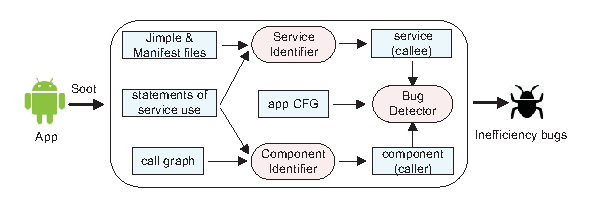
\includegraphics[scale=1.1]{framework.eps}
 \caption{Approach framework of \textsf{ServDroid}.}
\label{fig_framework}
\end{figure}

\subsection{Detecting Service Leak Bugs}
Normally, to bind a service, each bind statement should have a corresponding
unbind statement such that the callers (client components) of the two statements
are the same; however to start a service, multiple start statements may
correspond to the same stop statement. If a start (bind) statement is not always
followed by a stop (unbind) statement, the service may leak. As aforesaid, no
matter whether end users can destroy a service or not, the app itself should
have the mechanism to destroy the created service.  With this in mind, we have
the following steps to determine whether a service may leak or not:

\begin{table*}
\centering
\small
\caption{Popular Android apps studied in our experiments}
\begin{tabular}{|l|c|c|c|cccc|}\hline
{\bf App name}&{\bf Developer}&{\bf Category}&{\bf Version}&\multicolumn{4}{|c|}{\textbf{\#  Services}}\\
&  & & &{\bf Started}&{\bf Bound}&{\bf Hybrid} &{\bf Total}\\\hline
\hline
{\it Google Play services}&Google&Tools&11.0.55 (436-156917137)&{\bf 130}&{\bf 17}&6&{\bf 153}\\
{\it Gmail}&Google&Communication&7.6.4.158567011.release&18&1&4&23\\
{\it Maps}&Google&Travel \& Local&9.54.1&12&9&4&25\\
{\it YouTube}&Google&Video Players \& Editors&12.23.60&10&2&3&15\\
{\it Facebook}&Facebook&Social&10.2.0&22&8&4&34\\
{\it Google}&Google&Tools&7.3.25.21.arm&21&10&6&37\\
{\it Google+}&Google&Social&9.14.0.158314320&23&1&4&28\\
{\it GoogleText-to-Speech}&Google&Tools&3.11.12&3&0&0&3\\
{\it WhatsApp Messenger}&Facebook&Communication&2.17.231&9&4&3&16\\
{\it Google Play Books}&Google&Books \& Reference&3.13.17&8&2&1&11\\
{\it Messenger}&Facebook&Communication&123.0.0.11.70&40&1&0&41\\
{\it Hangouts}&Google&Communication&20.0.156935076&11&9&2&22\\
{\it Google Chrome}&Google&Communication&58.0.3029.83&16&9&2&27\\
{\it Google Play Games}&Google&Entertainment&3.9.08(3448271-036)&1&0&0&1\\
{\it Google TalkBack}&Google&Tools&5.2.0&2&1&0&3\\
{\it Google Play Music}&Google&Music \& Audio&7.8.4818-1.R.4063206&15&3&4&22\\
{\it Google Play Newsstand}&Google&News \& Magazines&4.5.0&8&1&0&9\\
{\it Google Play Movies \& TV}&Google&Video Players \& Editors&3.26.5&5&4&2&11\\
{\it Google Drive}&Google&Productivity&2.7.153.14.34&6&6&3&15\\
{\it Samsung Push Service}&Samsung&Communication&1.8.02&11&0&0&11\\
{\it Instagram}&Facebook&Social&10.26.0&14&3&2&19\\
{\it Android System WebView}&Google&Tools&58.0.3029.83&8&2&0&10\\
{\it Google Photos}&Google&Photography&2.16.0.157775819&15&6&6&27\\
{\it Google Street View}&Google&Travel \& Local&2.0.0.157538376&3&3&2&8\\
{\it Skype}&Microsoft&Communication&8.0.0.44736&10&1&0&11\\
{\it Clean Master}&Cheetah Mobile&Tools&5.17.4&14&7&5&26\\
{\it Subway Surfers}&Kiloo Games&Games/Arcade&1.72.1&2&1&0&3\\
{\it Dropbox}&Dropbox,Inc&Productivity&50.2.2&8&3&1&12\\
{\it Candy Crush Saga}&King&Games/Casual&1.101.0.2&2&1&1&4\\
{\it Twitter}&Twitter&News \& Magazines&7.0.0&9&2&2&13\\
{\it LINE}&LINE Corporation&Communication&7.5.2&11&5&3&19\\
{\it HP Print Service Plugin}&HP Inc&Productivity&3.4-2.3.0&4&3&2&9\\
{\it Flipboard}&Flipboard&News \& Magazines&4.0.13&4&3&3&10\\
{\it Samsung Print Service Plugin}&Samsung&Productivity&3.02.170302&7&3&0&10\\
{\it Super-Bright LED Flashlight}&Surpax Technology Inc&Productivity&1.1.7&3&0&2&5\\
{\it Gboard}&Google&Tools&6.3.28.159021150&6&4&2&12\\
{\it Cloud Print}&Google&Productivity&1.36b&7&1&1&9\\
{\it Snapchat}&Snap Inc&Social&10.10.5.0&2&0&0&2\\
{\it Pou}&Zakeh&Games/Casual&1.4.73&4&0&0&4\\
{\it Google Translate}&Google&Tools&5.9.0.RC07.155715800&6&0&1&7\\
{\it My Talking Tom}&Outfit7&Games/Casual&4.2.1.50&17&6&2&25\\
{\it Security Master}&Cheetah Mobile&Tools&3.4.1&7&3&4&14\\
{\it Facebook Lite}&Facebook&Social&20.0.15&20&9&4&33 \\
{\it imo messenger}&imo.im&Communication&11.3.2&16&6&{\bf 7}&29\\
\hline
{\bf Sum}& - & -& -& 578 &167  &  99 &  844\\
\hline
{\bf Average}&-&-&-&12.8 &  3.7 &  2.2 &  18.8\\
\hline
\end{tabular}
\label{tab_benchmark}
\end{table*}

\begin{enumerate}
\item We first find all statements that start (bind) the service, i.e., \hytt{startService()} (\hytt{bindService()}). All the  statements are summarized in a set $S_1$.
\item We then find all statements that stop (unbind) the service, i.e., \hytt{stopService()} (\hytt{unbindService()}). All the  statements are summarized in a set $S_2$.
\item We next remove from $S_2$ the statements that are triggered by end users, i.e., the statements that are in the event handlers (callbacks) of the UI events (e.g., user click).
\item For each start (bind) statement in $S_1$, i.e., \hytt{startService()} (\hytt{bindService()}), we check whether or not the corresponding stop (unbind) statement, i.e., \hytt{startService()} (\hytt{unbindService()}) exists in $S_2$. If not, the use of the service will lead to service leak. If yes, we further determine whether or not the stop (unbind) statement can be always reached from the corresponding start (bind) statement.  If not, the use of the service will also lead to service leak.
\end{enumerate}

In the last step above, it is challenging to determine whether a stop (unbind)
statement $stm_2$ can always be reached from the corresponding start (bind)
statement $stm_1$. Symbolic analysis can be used to precisely solve this
problem, but it is difficult to scale. To balance precision and scalability, our
method of determining service leak is based on the concept of
\textit{post-dominator} (cf. Definition~\ref{def_postdom}): if $stm_2$ is the
post-dominator of $stm_1$ (i.e., $stm_1$ is post-dominated by $stm_2$) in the
context-insensitive inter-procedure control flow graph of the app, then the
service does not leak. Otherwise, it may leak.

\begin{definition}[\textbf{Post-dominance and Post-dominator}]
  In a control flow graph, a node (statement) $s_i$ is post-dominated by another
  node (statement) $s_j$ if each directed path from $s_i$ to the exit (return
  statement) of the control flow graph contains $s_j$. $s_j$ is called a
  post-dominator of $s_i$.
\label{def_postdom}
\end{definition}


\section{Empirical Evaluation}\label{evaluation}
In this section, we conduct an empirical study on service usage inefficiencies in real-world popular Android apps, aiming at answering the following five research questions:

\begin{itemize}
\item {\bf RQ1} - {\it Service usage frequency}: Are background services widely used in Android apps? Which type of services is the most frequently-used?
\item {\bf RQ2} - {\it Pervasiveness of efficiency bugs}: Are service usage efficiency bugs common in practice?
\item {\bf RQ3} - {\it Distribution of efficiency bugs}: How are the four kinds of service usage efficiency bugs distributed in the three types of services?
\item {\bf RQ4} - {\it Dominating efficiency bugs}: Among the four kinds of service usage efficiency bugs, which kind is the most prevalent?
\item {\bf RQ5} - {\it Most vulnerable service type}: Among the three types of services, the usage of which type is more prone to efficiency bugs?
\end{itemize}

\subsection{Experimental Setup}

To facilitate our empirical analysis, we implement our approach in an open-source prototype tool {\sf ServDroid} based on {\sf Soot}~\cite{sootpaper}. The input of {\sf ServDroid} is an app (APK file), and its output is the detected service usage efficiency bugs in the app. If the use of a service is detected to involve efficiency bugs, the corresponding callers of the service are also outputted, which facilitates debugging. We apply {\sf ServDroid}) to 45 the most downloaded free Android apps according to Wikipedia. The first 25 apps are all with over one billion downloads and the rest 20 apps all have over 500 million downloads. Table~\ref{tab_benchmark} summarizes the basic information of these 45 apps, including the app names, developers, versions, and the number of services (smaller than that declared in the AndroidManifest file) implemented or used in the apps. It is worth mentioning that all the app versions are the latest in the early January, 2018.

Our experiment was performed on a computer with an Intel Core i7 3.6GHz CPU and 16 GB of memory, running Windows 8, JDK 1.7, and Android 7.0, 7.1.1, and 8.0.  The total runtime overhead of our prototype tool {\sf ServDroid} on analyzing the 45 apps is 4,293 seconds, with 95.4 seconds on average to analyze one app, which demonstrates the efficiency of {\sf ServDroid}.


\begin{table}
\centering
\footnotesize
\caption{Total number of service usage efficiency bugs}
\begin{tabular}{|l|ccccc|}\hline
{\bf App name}&\multicolumn{5}{|c|}{\textbf{Service usage inefficiency bugs}}\\
& {\bf \# PCBs}&{\bf \# LDBs}&{\bf \# PDBs} &{\bf \# SLBs}&{\bf Total}\\
\hline
\hline
{\it Google Play services}&2&3&0&{\bf 93}&{\bf 98}\\
{\it Gmail}&0&1&0&5&6\\
{\it Maps}&1&1&1&9&12\\
{\it YouTube}&0&1&0&3&4\\
{\it Facebook}&0&5&0&5&10\\
{\it Google}&0&3&0&1&4\\
{\it Google+}&0&1&0&7&8\\
{\it GoogleText-to-Speech}&0&0&0&2&2\\
{\it WhatsApp Messenger}&{\bf 4}&2&{\bf 3}&10&19\\
{\it Google Play Books}&0&0&0&1&1\\
{\it Messenger}&0&1&0&9&10\\
{\it Hangouts}&0&1&1&3&5\\
{\it Google Chrome}&0&0&0&0&0\\
{\it Google Play Games}&0&0&0&3&3\\
{\it Google TalkBack}&0&0&0&1&1\\
{\it Google Play Music}&0&2&2&10&14\\
{\it Google Play Newsstand}&0&1&1&3&5\\
{\it Google Play Movies \& TV}&0&0&0&4&4\\
{\it Google Drive}&0&2&0&3&5\\
{\it Samsung Push Service}&0&3&0&1&4\\
{\it Instagram}&0&1&0&7&8\\
{\it Android System WebView}&0&0&0&0&0\\
{\it Google Photos}&1&2&1&4&8\\
{\it Google Street View}&0&5&0&6&11\\
{\it Skype}&0&0&0&0&0\\
{\it Clean Master}&0&{\bf 12}&2&25&39\\
{\it Subway Surfers}&0&0&0&1&1\\
{\it Dropbox}&1&1&1&4&7\\
{\it Candy Crush Saga}&0&1&0&0&1\\
{\it Viber Messenger}&1&2&0&5&8\\
{\it Twitter}&0&1&0&3&4\\
{\it LINE}&1&1&1&11&14\\
{\it HP Print Service Plugin}&0&1&0&4&5\\
{\it Flipboard}&0&1&0&2&3\\
{\it Samsung Print Service Plugin}&0&3&0&6&9\\
{\it Super-Bright LED Flashlight}&0&2&0&7&9\\
{\it Gboard}&0&0&0&1&1\\
{\it Cloud Print}&0&2&0&1&3\\
{\it Snapchat}&0&5&0&2&7\\
{\it Pou}&0&2&0&2&4\\
{\it Google Translate}&0&4&0&3&7\\
{\it My Talking Tom}&0&3&2&15&20\\
{\it Security Master}&2&1&2&7&12\\
{\it Facebook Lite}&1&9&2&7&19 \\
{\it imo messenger}&2&4&1&14&21\\
\hline
{\bf Sum}&16&90&20&310&436\\
\hline
{\bf Average}&0.4&2.0&0.4&6.8&9.6\\
\hline
\end{tabular}
\label{tab_resultsum}
\end{table}

\subsection{Experimental Results}
The last columns of Table~\ref{tab_benchmark} summarize the numbers of different types of services used in the 45 Android apps. From these results, we have the following finding:

\medskip
%\setlength{\fboxrule}{0.7 pt}
%\setlength{\fboxsep}{0.2 cm}
{\setlength{\parindent}{0 em}
\fbox{\begin{minipage}{3.23 in}
{\bf Finding~1:}
All 45 apps use background services. The total numbers (proportions) of started, bound, and hybrid services in these apps are 578 (68.48\%), 167 (19.79\%), and 99 (11.73\%), respectively. Each app uses 18.8 services on average. The average numbers of started, bound, and hybrid services used in an app are 12.8, 3.7, and 2.2, respectively.\\
{\bf Implication:}
Services are widely used in Android apps.
Started services are the most frequently-used type of services.
\end{minipage}}
}\\
\medskip

The reason why started services are the most-frequently used type of services lies in that they require less user interaction, and are thus particularly suitable for time-consuming tasks running on the background.

Table~\ref{tab_resultsum} summarizes the total number of detected service usage efficiency bugs in these apps. Table~\ref{tab_result} reports on the numbers of premature create bugs (PCBs), late destroy bugs (LDBs), premature destroy bugs (PDBs), and service leak bugs (SLBs) with respect to the started, bound, and hybrid services in the 45 Android apps, respectively. In summary, we have the following findings:

\medskip
%\setlength{\fboxrule}{0.7 pt}
%\setlength{\fboxsep}{0.2 cm}
{\setlength{\parindent}{0 em}
\fbox{\begin{minipage}{3.23 in}
{\bf Finding~2:}
Surprisingly, service usage efficiency bugs are common in the 45 Android apps. 42 (93.33\%) of them are infected by at least one kind of efficiency bugs; 34 (75.56\%) of them involve at least two kinds of efficiency bugs; 15 (33.33\%) of them have no less than three kinds of efficiency bugs; and 8 (17.78\%) of them are found to have all the four kinds of efficiency bugs. \\
{\bf Implication:}
Service usage efficiency bugs are common in real-world popular Android apps.
\end{minipage}}
}\\
\medskip


\medskip
%\setlength{\fboxrule}{0.7 pt}
%\setlength{\fboxsep}{0.2 cm}
{\setlength{\parindent}{0 em}
\fbox{\begin{minipage}{3.23 in}
{\bf Finding~3:}
The numbers (proportions) of premature create bugs occurring on the started services, bound services, and hybrid services are 0 (0\%), 0 (0\%), and 16 (100\%), respectively. The numbers (proportions) of late destroy bugs occurring on the started services, bound services, and hybrid services are 27 (30\%), 48 (53.33\%), and 15 (16.67\%), respectively. The numbers (proportions) of premature destroy bugs occurring on the started services, bound services, and hybrid services are 14 (70\%), 0 (0\%), and 6 (30\%), respectively. The numbers (proportions) of service leak bugs occurring on the started services, bound services, and hybrid services are 231 (74.52\%), 32 (10.32\%), and 47 (15.16\%), respectively.\\
{\bf Implication:}
This confirms the conclusion in Table~\ref{tab_correlation} that the premature create bugs only happen to the usage of hybrid services; premature destroy bugs do not occur on the usage of bound services; late destroy bugs and service leak bugs can happen to all the three types of services.
\end{minipage}}
}\\
\medskip

\medskip
%\setlength{\fboxrule}{0.7 pt}
%\setlength{\fboxsep}{0.2 cm}
{\setlength{\parindent}{0 em}
\fbox{\begin{minipage}{3.23 in}
{\bf Finding~4:}
Among the 45 apps, 10 (22.22\%) apps have premature create bugs,  35 (77.78\%) apps are infected by late destroy bugs; 13 (28.89\%) apps are found to have premature destroy bugs; and 41 (91.11\%) apps involve service leak bugs. \\
{\bf Implication:}
Service leak bugs and premature create bugs are the most and least prevalent kinds of service usage inefficiencies, respectively.
\end{minipage}}
}\\
\medskip

\medskip
%\setlength{\fboxrule}{0.7 pt}
%\setlength{\fboxsep}{0.2 cm}
{\setlength{\parindent}{0 em}
\fbox{\begin{minipage}{3.23 in}
{\bf Finding~5:}
The total numbers of premature create bugs,
late destroy bugs, premature destroy bugs, and service leak bugs in the 45 apps are 16, 90, 20, and 310, respectively. The proportions of the four kinds of service usage efficiency bugs are  3.67\%, 20.64\%, 4.59\%, and 71.10\%, respectively. Each app involves 9.6 service usage efficiency bugs on average. The average numbers of premature create bugs,
late destroy bugs, premature destroy bugs, and service leak bugs  in an app are 0.4, 2.0, 0.4, and 6.8, respectively.\\
{\bf Implication:}
The number of service leak bugs is much larger than the total number of the other three kinds of service usage efficiency bugs. Service leak bugs are the dominant kind of service usage inefficiencies.
\end{minipage}}
}\\
\medskip

Compared to the other three kinds of service usage efficiency bugs, the negative effects of service leak bugs are the biggest, because service leak bugs lead to more unnecessary memory occupation and energy consumption. The conclusion of Findings~4 and~5 indicate that service leak bugs are the most severe kind of service usage inefficiencies in apps.



\medskip
%\setlength{\fboxrule}{0.7 pt}
%\setlength{\fboxsep}{0.2 cm}
{\setlength{\parindent}{0 em}
\fbox{\begin{minipage}{3.23 in}
{\bf Finding~6:}
272 service usage efficiency bugs are relevant to the usage of 578 started services, 80 service usage efficiency bugs happen to the usage of 167 bound services, and 84 service usage efficiency bugs occur on the usage of 99 hybrid services.  \\
{\bf Implication:}
Among the three types of services, the usage of hybrid services has the highest possibility to involve efficiency bugs, whereas the usage of started services and bound services has the lower possibilities to involve efficiency bugs.
\end{minipage}}
}\\
\medskip

%We also applied \textsf{ServDroid} to other 60 real-world but not so popular Android apps, and found that those apps involve even more service usage efficiency bugs. 
We have also applied \textsf{ServDroid} to different versions of some apps, and find that, the numbers of service usage efficiency bugs decrease with the increasing app versions (cf. Figure~\ref{fig_bugsvsversions}). This implies that some developers fixed such bugs, though not completely. In summary, our empirical study indicate that service usage efficiency bugs are pervasive in Android apps, and most developers have not yet been aware of the severity.

\begin{table*} [htbp]
\centering
\small
\caption{The number of service usage efficiency bugs occurring to different types of services}
\begin{tabular}{|l|cccc|ccc|ccccc|}\hline
{\bf App name}&\multicolumn{4}{|c|}{\textbf{Started service}}&\multicolumn{3}{|c|}{\textbf{Bound services}}&\multicolumn{5}{|c|}{\textbf{Hybrid services}}\\
& {\bf \# LDBs}&{\bf \# PDBs} &{\bf \# SLBs}&{\bf Total}
& {\bf \# LDBs}& {\bf \# SLBs}&{\bf Total}
& {\bf \# PCBs}&{\bf \# LDBs}&{\bf \# PDBs} &{\bf \# SLBs}&{\bf Total}\\
\hline
\hline
{\it Google Play services}&1&0&{\bf 90}&{\bf 91}&2&0&2&2&0&0&3&5\\
{\it Gmail}&1&0&4&5&0&1&1&0&0&0&0&0\\
{\it Maps}&0&0&6&6&1&0&1&1&0&1&3&5\\
{\it YouTube}&0&0&3&3&1&0&1&0&0&0&0&0\\
{\it Facebook}&3&0&5&8&2&0&2&0&0&0&0&0\\
{\it Google}&1&0&0&1&2&1&3&0&0&0&0&0\\
{\it Google+}&0&0&7&7&1&0&1&0&0&0&0&0\\
{\it Google Text-to-Speech}&0&0&2&2&0&0&0&0&0&0&0&0\\
{\it WhatsApp Messenger}&0&{\bf 2}&2&4&2&0&2&{\bf 4}&0&1&{\bf 8}&{\bf 13}\\
{\it Google Play Books}&0&0&1&1&0&0&0&0&0&0&0&0\\
{\it Messenger}&1&0&9&10&0&0&0&0&0&0&0&0\\
{\it Hangouts}&0&1&0&1&1&1&2&0&0&0&2&2\\
{\it Google Chrome}&0&0&0&0&0&0&0&0&0&0&0&0\\
{\it Google Play Games}&0&0&3&3&0&0&0&0&0&0&0&0\\
{\it Google TalkBack}&0&0&1&1&0&0&0&0&0&0&0&0\\
{\it Google Play Music}&1&0&2&3&0&{\bf 3}&3&0&1&{\bf 2}&5&8\\
{\it Google Play Newsstand}&1&1&3&5&0&0&0&0&0&0&0&0\\
{\it Google Play Movies \& TV}&0&0&4&4&0&0&0&0&0&0&0&0\\
{\it Google Drive}&0&0&3&3&2&0&2&0&0&0&0&0\\
{\it Samsung Push Service}&1&0&0&1&2&1&3&0&0&0&0&0\\
{\it Instagram}&1&0&3&4&0&{\bf 3}&3&0&0&0&1&1\\
{\it Android System WebView}&0&0&0&0&0&0&0&0&0&0&0&0\\
{\it Google Photos}&0&1&3&4&1&0&1&1&1&0&1&3\\
{\it Google Street View}&2&0&2&4&1&0&1&0&2&0&4&6\\
{\it Skype}&0&0&0&0&0&0&0&0&0&0&0&0\\
{\it Clean Master}&1&{\bf 2}&15&18&{\bf 8}&{\bf 3}&{\bf 11}&0&{\bf 3}&0&7&10\\
{\it Subway Surfers}&0&0&0&0&0&1&1&0&0&0&0&0\\
{\it Dropbox}&0&1&1&2&1&2&3&1&0&0&1&2\\
{\it Candy Crush Saga}&0&0&0&0&1&0&1&0&0&0&0&0\\
{\it Viber Messenger}&0&0&4&4&1&1&2&1&1&0&0&2\\
{\it Twitter}&1&0&2&3&0&1&1&0&0&0&0&0\\
{\it LINE}&0&1&6&7&1&2&3&1&0&0&3&4\\
{\it HP Print Service Plugin}&0&0&3&3&1&1&2&0&0&0&0&0\\
{\it Flipboard}&0&0&1&1&1&1&2&0&0&0&0&0\\
{\it Samsung Print Service Plugin}&0&0&5&5&3&1&4&0&0&0&0&0\\
{\it Super-Bright LED Flashlight}&0&0&5&5&1&1&2&0&1&0&1&2\\
{\it Gboard}&0&0&1&1&0&0&0&0&0&0&0&0\\
{\it Cloud Print}&0&0&1&1&2&0&2&0&0&0&0&0\\
{\it Snapchat}&2&0&2&4&2&0&2&0&1&0&0&1\\
{\it Pou}&2&0&2&4&0&0&0&0&0&0&0&0\\
{\it Google Translate}&1&0&2&3&1&1&2&0&2&0&0&2\\
{\it My Talking Tom}&1&1&11&13&2&2&4&0&0&1&2&3\\
{\it Security Master}&0&1&3&4&0&2&2&2&1&1&2&6\\
{\it Facebook Lite}&{\bf 4}&{\bf 2}&4&10&3&1&4&1&2&0&2&5\\
{\it imo messenger}&2&1&10&13&2&2&4&2&0&0&2&4\\
\hline
{\bf Sum}&27&14&231&272&48&32&80&16&15&6&47&84\\
\hline
{\bf Average}&0.6&0.3&5.1&6.0&1.1&0.7&1.8&0.4&0.3&0.1&1.0&1.8\\
\hline
\end{tabular}\label{tab_result}
\end{table*}

%\begin{figure}
%  \centering
%  \subfigure[]{
%    \includegraphics[scale=0.5]{bugs_vs_versions.eps}}
%  \subfigure[]{
%    \includegraphics[scale=0.5]{bound.eps}}
%  \caption{The number of services usage efficiency bugs decreases with increasing app versions.}
%\label{fig_lifecycle}
%\end{figure}

 \begin{figure}
 \centering
  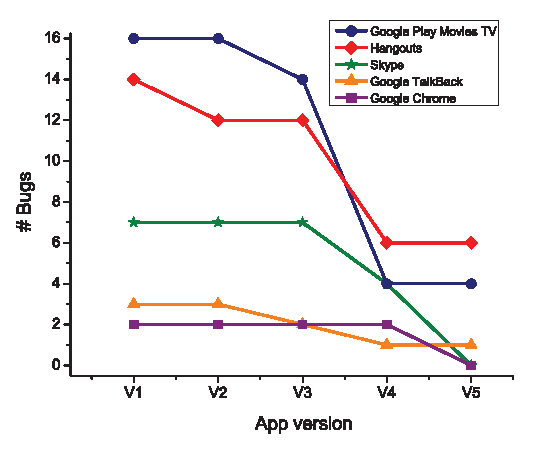
\includegraphics[scale=0.4]{bugs-vs-versions.eps}
 \caption{The number of services usage efficiency bugs decreases with the increasing app version, where concrete version numbers are abstracted away.}
\label{fig_bugsvsversions}
\end{figure}

\subsection{Case Studies}
In this part, we reports on some service usage efficiency bugs detected from three Android apps.

\textbf{YouTube} is a well-known video-sharing platform all over the world. For its Android app of version 12.23.60, the number of started, bound, and hybrid services implemented or used in \textit{YoutTube} is ten, two, and three, respectively. Our tool \textsf{ServDroid} finds totally four service usage efficiency bugs from this app. The code snippet in Figure~\ref{YouTube}a shows a late destroy bug found in this app, where the class \hytt{ahx} binds a service from a third party. The \hytt{bindService()} method is called in the \hytt{d()} method of \hytt{ahx}, but the corresponding \hytt{unbindService()} method is not immediately called after the last invocation of the method (i.e.,\hytt{post()}) of the service in \hytt{f()}. The service remains idle until the \hytt{e()} method of \hytt{ahx} is called. The code snippet in Figure~\ref{YouTube}b exhibits a service leak bug found from \textit{YoutTube}: The \hytt{startService()} method that starts \hytt{AnalyticsService} is called in the \hytt{onReceive} method of \hytt{jth}, but no \hytt{stopSelf()} or \hytt{stopService()} exists to stop \hytt{AnalyticsService}.

\begin{figure}
  \centering
  \subfigure[]{
    \lstinputlisting[language={Java}]{YouTube_LDB.java}}
  \subfigure[]{
    \lstinputlisting[language={Java}]{YouTube_SLB.java}}
  \caption{Service usage efficiency bugs in \textit{YouTube} (version 12.23.60): (a) A late destroy bug, (b) A service leak bug.}
\label{YouTube}
\end{figure}

\begin{figure}
  \centering
  \subfigure[]{
    \lstinputlisting[language={Java}]{WhatsAppMessenger_PCB.java}}
  \subfigure[]{
    \lstinputlisting[language={Java}]{WhatsAppMessenger_LDB.java}}
  \subfigure[]{
    \lstinputlisting[language={Java}]{WhatsAppMessenger_PDB.java}}
  \subfigure[]{
    \lstinputlisting[language={Java}]{WhatsAppMessenger_SLB.java}}
  \caption{Service usage efficiency bugs in \textit{WhatsApp Messenger} (version 2.17.231): (a) A premature create bug, (b) A late destroy bug, (c) A premature destroy bug, (d) A service leak bug.}
\label{WhatsAppMessenger}
\end{figure}

\textbf{WhatsApp Messenger} is a popular mobile messaging app that allows people to exchange messages using the devices' Internet connections. For its version 2.17.231, the number of started, bound, and hybrid services implemented or used in \textit{WhatsApp Messenger} is nine, four, and three, respectively. Although the service quantity is not large, 19 service usage efficiency bugs are found by our tool \textsf{ServDroid}, including four premature create bugs, two late destroy bugs, three premature destroy bugs, and 10 service leak bugs. The code snippet in Figure~\ref{WhatsAppMessenger}a reports a premature create bug in this app: The \hytt{onStartCommand()} method of the \hytt{GoogleDriveService} is not overwritten, and the \hytt{bindService} method is called after (but not immediately) the \hytt{startService} method. The code snippet in Figure~\ref{WhatsAppMessenger}b shows a late destroy bug, where \hytt{SearchActionVerificationClientService} binds a remote service from Google. The \hytt{bindService()} method is called in the \hytt{onCreate()} method of \hytt{SearchActionVerificationClientService}, but the corresponding \hytt{unbindService()} method is not immediately called after the last invocation of the method \hytt{isSearchAction()} of the Google service in \hytt{onHandleIntent()}. The Google service remains idle until the \hytt{onDestroy()} method of the \hytt{SearchActionVerificationClientService} is called. The code snippet in Figure~\ref{WhatsAppMessenger}c corresponds to a premature destroy bug: The \hytt{startService()} method of  \hytt{MessageService} is called three times, but the \hytt{stopSelf()} (instead of \hytt{stopSelf(int)}) method is used in the \hytt{onStartCommand()} method of \hytt{MessageService}. The code snippet in Figure~\ref{WhatsAppMessenger}d exhibits a service leak bug: The \hytt{startService()} method that starts \hytt{ExternalMediaManager} is called in the \hytt{onReceive} method of \hytt{ExternalMediaStateReceiver}, but no \hytt{stopSelf()} or \hytt{stopService()} exists to stop \hytt{ExternalMediaManager}.

\begin{figure}
  \centering
  \subfigure[]{
    \lstinputlisting[language={Java}]{Twitter_LDB.java}}
  \subfigure[]{
    \lstinputlisting[language={Java}]{Twitter_SLB.java}}
  \caption{Service usage efficiency bugs in \textit{Twitter} (version 7.0.0): (a) A late destroy bug, (b) A service leak bug.}
\label{Twitter}
\end{figure}


\textbf{Twitter} is an app designed to reduce busywork, which allows users to focus on the things that matter. For its version 7.0.0, the number of started, bound, and hybrid services implemented or used in \textit{Twitter} is nine, two, and two, respectively. Although the number of services is not large, four service usage efficiency bugs are detected by our tool \textsf{ServDroid}, including one late destroy bug and three service leak bugs. The code snippet in Figure~\ref{Twitter}a reports the late destroy bug, where the \hytt{a()} method starts a service \hytt{OverlayService}. Despite the fact that the \hytt{stopService()} method is called in the \hytt{b()} method, the time to stop the \hytt{OverlayService} is too late. To address this problem, the \hytt{stopSelf()} method should be invoked in the \hytt{onStartCommand()} method of \hytt{OverlayService}. The code snippet in Figure~\ref{Twitter}b shows a service leak bug found from \textit{Twitter}: The \hytt{startService()} method that starts the service \hytt{OemHelperService} is called in the \hytt{a()} method of the class \hytt{OemIntentReceiver}, but,  surprisingly, there is no \hytt{stopSelf()} or \hytt{stopService()} available in the app code to stop \hytt{OemHelperService}.

%Similar service usage efficiency bugs are found in other 42 Android apps used in our study. The reason why service usage efficiency bugs are so prevalent is that their effects are not so severe as those of the functional bugs, that is, they do not cause app crashes, and thus developers do not regard them as a tricky problem.



\section{Related Work}\label{relatedwork}
Our research is related to the work on GUI testing, service  analysis and testing, and performance (energy) testing of Android apps. In the following, we review the state-of-the-art of these there aspects.

\textbf{GUI testing}. Most existing testing approaches for Android apps focus on GUI testing. According to the exploration strategies employed, Choudhary et al.~\cite{ChoudharyGO15} summarize three main categories of testing approaches: \textit{random testing}~\cite{monkey,HuN11,MachiryTN13,SongQH17}, \textit{model-based testing}~\cite{GUIRipping,grey-box,ChoiNS13,a3e,SuMCWYYPLS17}, and \textit{advanced testing}~\cite{AnandNHY12,JensenPM13,EvoDroid,MaoHJ16}. Although \textsf{Monkey}~\cite{monkey} is among the first generation techniques for Android testing, compared with many follow-up approaches, it still shows good performance and advantages in app testing~\cite{ChoudharyGO15}. \textsf{Dynodroid}~\cite{MachiryTN13} improves \textsf{Monkey} by reducing the possibility of generating redundant events. It achieves this by monitoring the reaction of an app upon each event and basing on the reaction to generate the next event. Recently, \textsf{EHBDroid}~\cite{SongQH17} is presented to first instrument the invocations of event callbacks in each activity and then directly trigger the callbacks in a random order. This approach is more efficient as it bypasses the GUI for test input generation. Since random testing may generate redundant events, several model-based testing approaches are proposed~\cite{AmalfitanoFT11,GUIRipping,grey-box,ChoiNS13,a3e,BaekB16,SuMCWYYPLS17}. These approaches first obtain a model of the app GUI, and then generate test input according to the model. While most of them utilize program analysis techniques to obtain the model, machine learning is used in~\cite{ChoiNS13} to learn the model. The third category approaches leverage advanced techniques to efficiently generate effective event sequences for app testing\cite{AnandNHY12,JensenPM13,EvoDroid,MaoHJ16}. For example,  \textsf{ACTEve}~\cite{AnandNHY12} uses symbolic execution and \textsf{EvoDroid}~\cite{EvoDroid} employs evolutionary algorithm to generate event sequences. \textsf{Sapienz}~\cite{MaoHJ16} formulates the event sequence generation as a multiple-objective optimization problem and employs search-based algorithm to generate the shortest event sequences that can maximize the code coverage and bug exposure.

\textbf{Service analysis and testing}. A deal of work concentrates on the security vulnerabilities (e.g., denial of service, single point failure) of Android system services~\cite{ReavesBGABCDHKS16,HuangZ0015,WangZL16,FengS16,AbualolaAKOM16,LuoZCCLLGYXL17}.
In terms of app services, Khanmohammadi et al. find that malware may use background services to perform malicious operations with no communication with the other components of the app~\cite{KhRH15}. They propose to use classification algorithms to differentiate normal and malicious apps based on the service features related to their lifecycle. In contrast to GUI testing for activities, background service testing gain little attention. \textsf{Snowdrop}~\cite{ZhangLLC17} is among the first to automatically and systematically testing background services in apps. Since not all \textit{Intent} messages can be directly derived from the app bytecode, \textsf{Snowdrop} infers field values based on a heuristic that leverages the similarity in how developers name variables. This approach can find general bugs (functional bugs that lead to app crashes) in services, but may meet difficulties in detecting service usage efficiency bugs targeted in this paper.

\textbf{Performance testing}. Non-functional or performance bugs in apps are also important for user experience. Liu et al.~\cite{LiuXC14} conduct an empirical study on 29 popular Android apps and find three types of performance bugs: GUI lagging, energy leak, and memory bloat. They also summarize common performance bug patterns (including lengthy operations in main threads, wasted computation for invisible GUI, and frequently invoked heavy-weight callbacks) and propose method to detect them. Since energy is a major concern in app performance and green software engineering~\cite{PangHAH16,HoqueSKXT16,MBZSJSPC16,0036990}, energy bugs and the corresponding testing solutions draw increasing attention~\cite{GuoZYZZ13,BanerjeeC0R14,LiuXCL14,BehrouzSBM16,WuYR16,JabbarvandM17}.   It is worth mentioning that energy bugs are highly relevant to resource leak~\cite{GuoZYZZ13,BanerjeeC0R14,LiuXCL14,WuYR16}. Banerjee et al. present a testing framework to detect energy bugs and energy hotspots in apps based on the measurement of the power consumption through a power meter. Although the framework also considers service leak bugs, the test oracle based on the power consumption is expensive and time-consuming. To reduce the cost of the test, Jabbarvand et al. propose an approach to minimize the energy-aware test-suite~\cite{BehrouzSBM16}. Wu et al. present a static analysis approach to detecting GUI-related energy-drain bugs~\cite{WuYR16}, whereas our approach aims to detect service usage efficiency bugs.

\section{Conclusions}\label{conclusion}
It is of great difficulty for testing techniques to reveal service usage efficiency bugs in Android apps, because such bugs do not cause apps to crash immediately. In this paper, we propose to use static analysis to address this problem. To this end, we first formulate four anti-patterns that lead to service usage efficiency bugs. Based on {\sf Soot}, we present the approach to detecting all such bugs in Android apps. To the best of our knowledge, our work is among the first to detect service performance bugs using static analysis. Our approach is implemented as an open-source tool {\sf ServDroid}, based on which, we conduct an empirical study. The empirical results demonstrate that service usage efficiency bugs are surprisingly pervasive in real-world popular apps, and the developers have not yet been aware of the severity of the bugs.

\bibliographystyle{ACM-Reference-Format}
\bibliography{ref}

\end{document}
